\section{Proposed Design}
\label{section:propeseddesign}

Before doing any implementation, we conducted some investigation into how Hadoop works, 
specifically how it assigns tasks initially and how they are reassigned during runtime.
These are important attributes to understand, because they contribute to uneven effective
workloads in a heterogeneous environment; that is, if two machines are assigned equal-sized
tasks, but one machine is twice as powerful as the other, it was effectively given half as
much work since it will complete it twice as fast as the other machine.

\subsection{Hadoop MapReduce Task Assignment}

We show the steps Hadoop MapReduce takes to carry out a job in \ref{fig:flow}. MapReduce 
works by taking map and reduce functions from the application (Wordcount for example), 
then configuring a \texttt{Job} object representing that application and its configuration.
Input data for the job is loaded into the Hadoop Distributed File System by the user. 
The job is then submitted to the \texttt{JobClient}, which subsequently calls the 
\texttt{getSplits} method to divide the input data to appropriate sizes to be sent out to
the MapReduce nodes. The \texttt{TaskTracker} on each slave node communicates with
the \texttt{JobTracker} on the master node to be assigned FileInput splits based on the
\texttt{TaskScheduler}.

\begin{figure}[ht!]
\centering
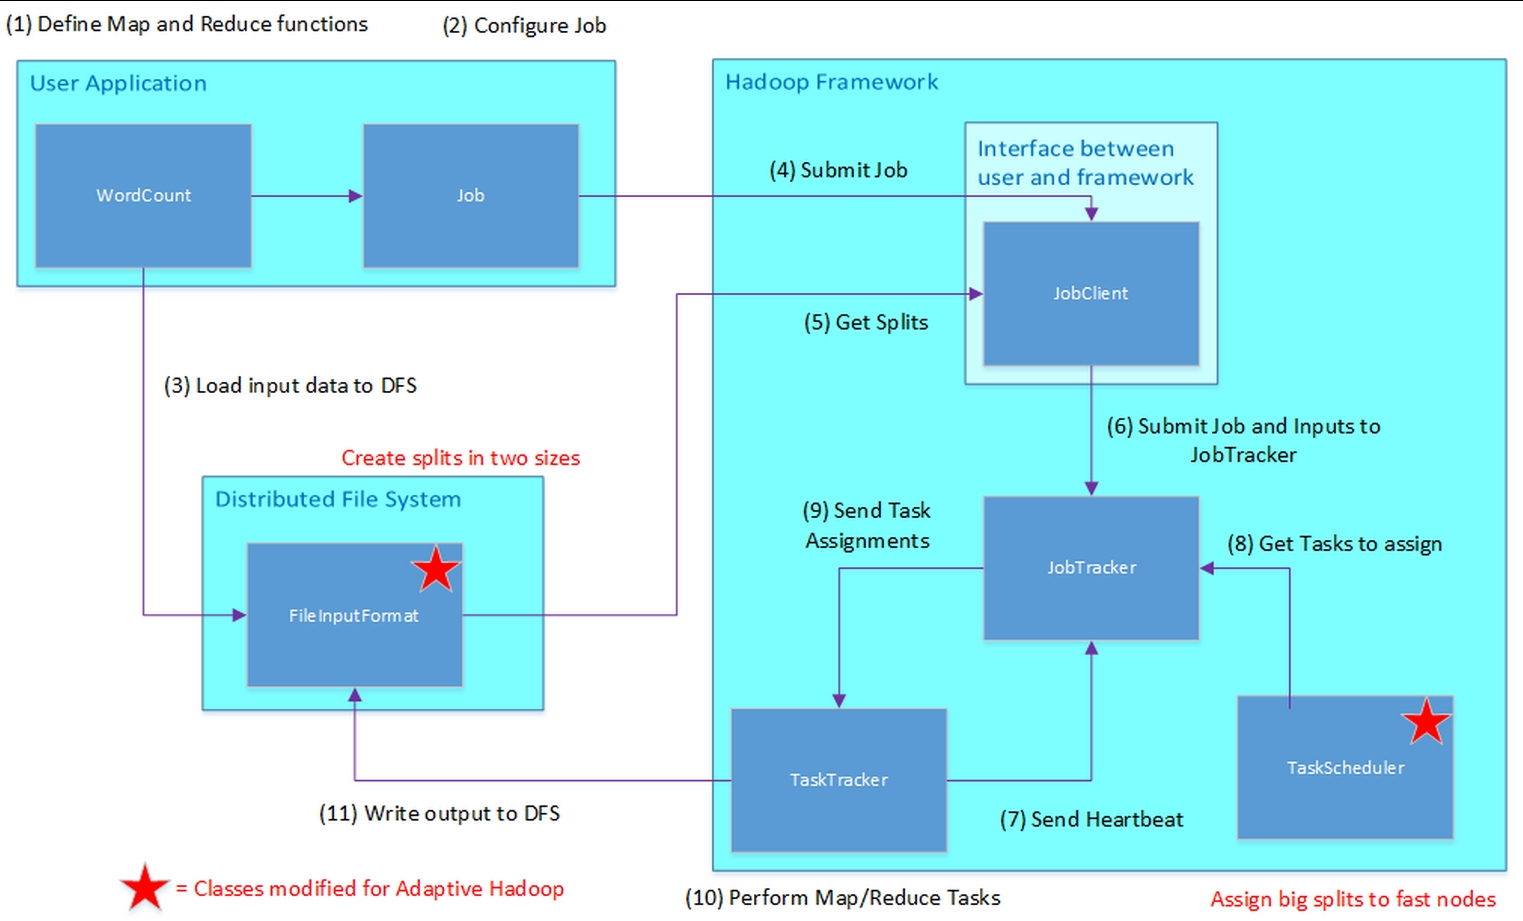
\includegraphics[width=90mm]{flow.jpg}
\caption{Workflow of a Hadoop MapReduce job}
\label{fig:flow}
\end{figure}

\begin{figure}[ht!]
\centering
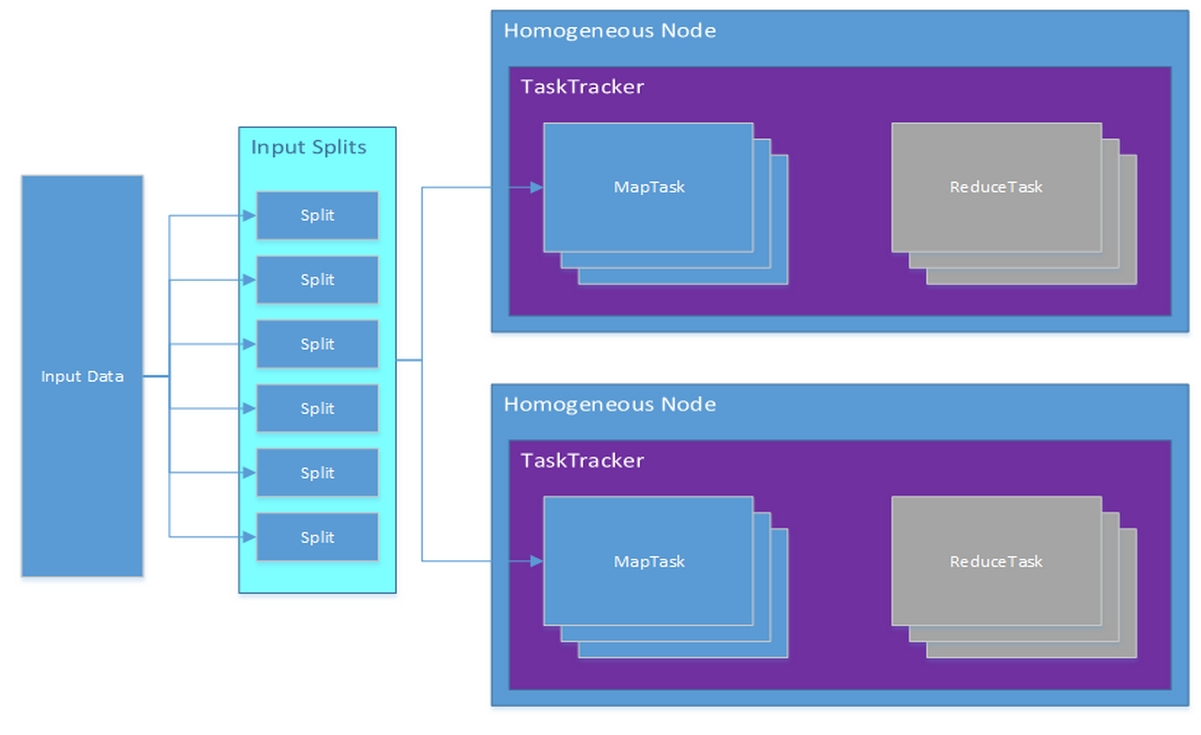
\includegraphics[width=90mm]{homogeneous_mr.jpg}
\caption{MapReduce task assignment in Homogeneous Environment}
\label{fig:homogeneoues_mr}
\end{figure}

\begin{figure}[ht!]
\centering
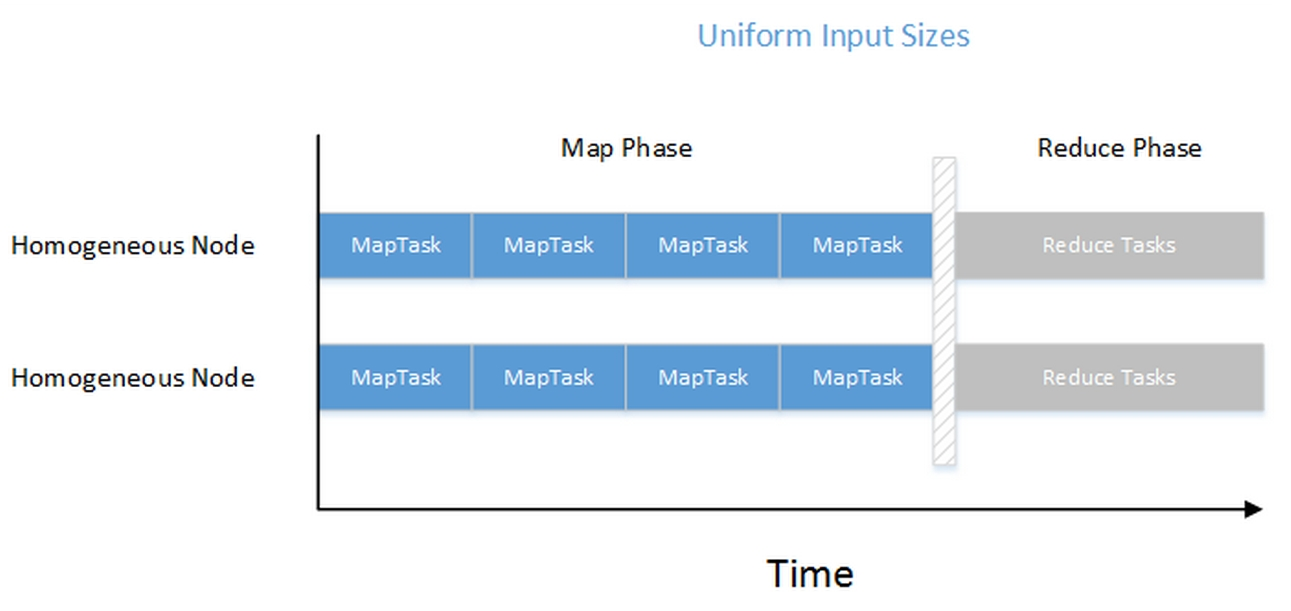
\includegraphics[width=90mm]{homogeneous_time.jpg}
\caption{MapReduce task completion in Homogeneous Environment}
\label{fig:homogeneoues_time}
\end{figure}

Hadoop MapReduce is designed for homogeneous environments. Without modifications, the input
data is divided into evenly-sized splits \ref{fig:homogeneous_mr}. In a homogeneous environment, 
this would be ideal since each node would be assigned the same number of map tasks, and would 
finish each one in the same amount of time, as shown in \ref{fig:homogeneous_time}. 

Modern datacenters, as we discussed in \ref{motivation}, are usually heterogeneous. That means,
when given the same amount of uniformly-sized tasks, different nodes will complete their tasks 
at different times. We show an example of this in \ref{fig:heterogeneous_time}. If the task completion
is skewed enough, the fastest nodes will actually steal tasks from the slower nodes; however,
this would introduce other performance issues from the overhead of the task stealing, and
sub-optimal performance from potential data locality issues. We believe a better solution is to
adjust the FileInput split sizes in proportion to the nodes' performance capabilities, such that
the total task completion time for each node is the same (\ref{adaptive_mr}). We could do this by making some larger
splits which would be assigned to the more powerful nodes. An example of this flow is shown in
\ref{adaptive_time} showing an example optimal adaptation.

\begin{figure}[ht!]
\centering
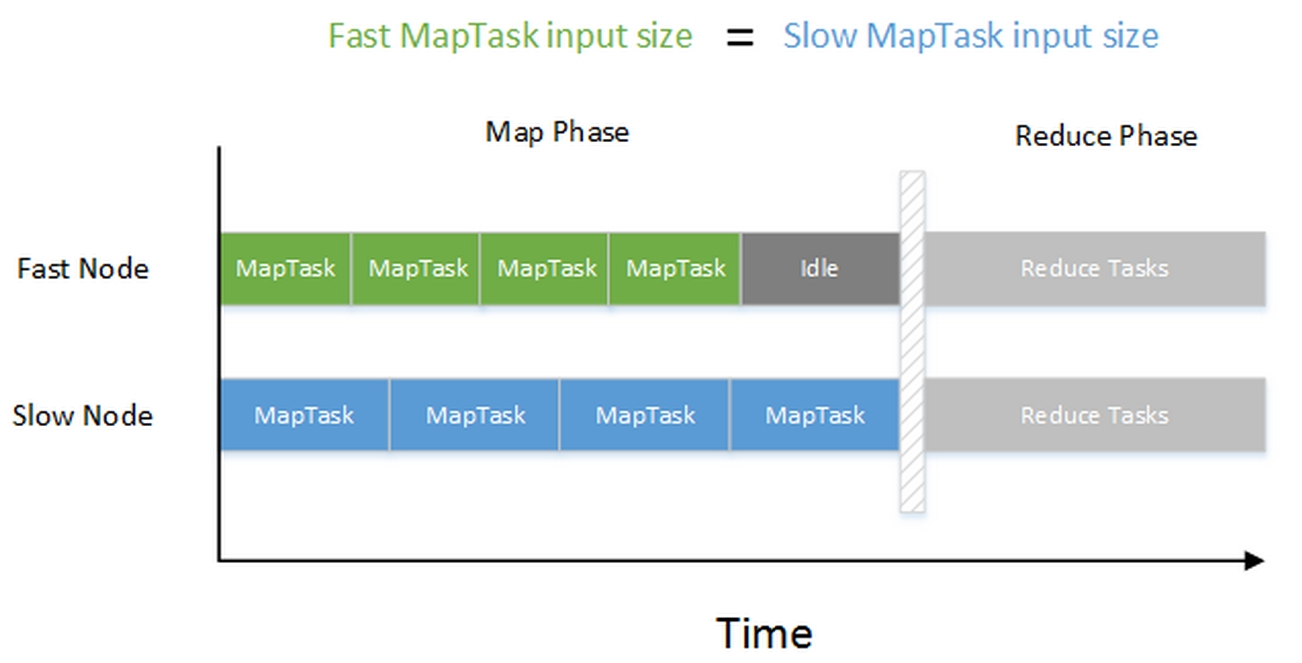
\includegraphics[width=90mm]{heterogeneous_time.jpg}
\caption{MapReduce task completion in Heterogeneous Environment}
\label{fig:heterogeneous_time}
\end{figure}

\begin{figure}[ht!]
\centering
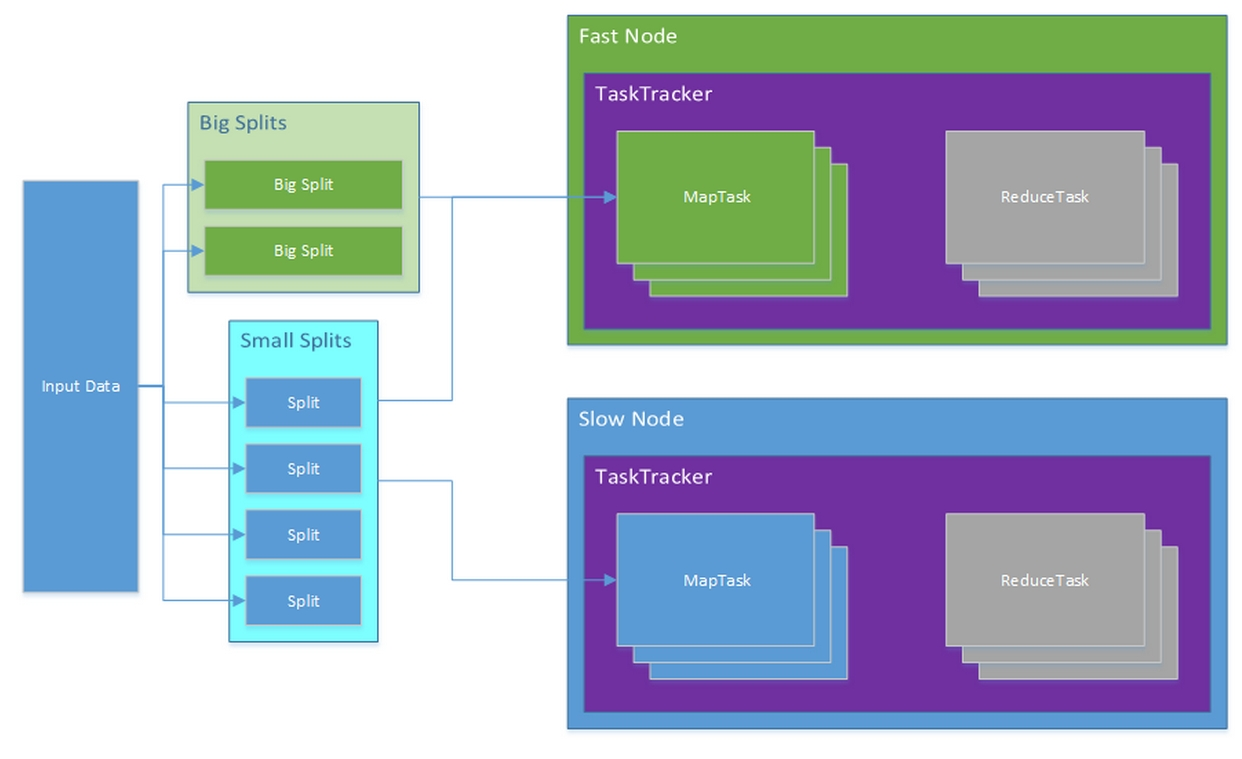
\includegraphics[width=90mm]{adaptive_mr.jpg}
\caption{MapReduce adapted flow for Heterogeneous Environment}
\label{fig:adaptive_mr}
\end{figure}

\begin{figure}[ht!]
\centering
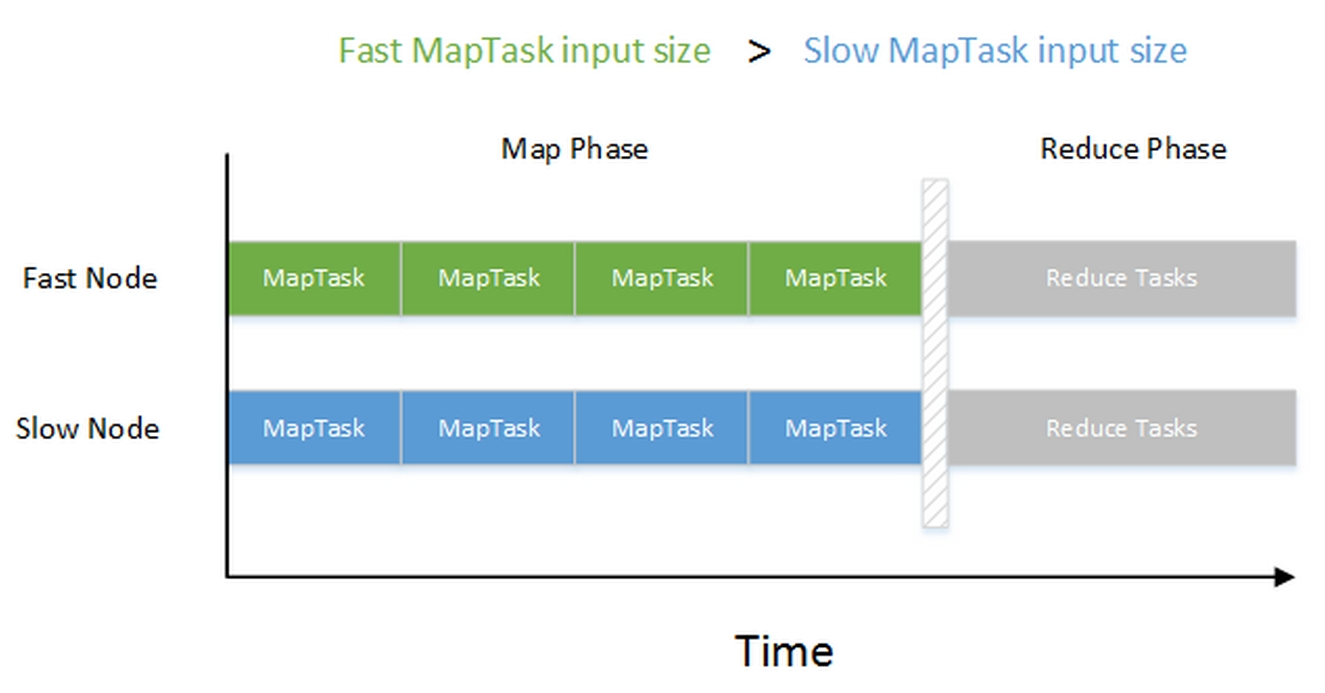
\includegraphics[width=90mm]{adaptive_time.jpg}
\caption{MapReduce task completion in Heterogeneous Environment with adaptive split sizes}
\label{fig:adaptive_time}
\end{figure}

\subsection{Datacenter VM Interference}
\label{sec:interference}
In addition to hetergeneous machines, datacenters can also exhibit temporal heterogeneity.
VM performance depends on the behavior of other VMs on the same machine at any given time.
This means a VM on a machine with other, inactive VMs will initially be very performant;
but once the other VMs begin doing work the VM will experience performance degradation.
The variability of a VM's performance also depends on the abstraction layer between the VMs
and the physical hardware.

\subsection{Hadoop MapReduce Task Stealing}
The hardware interefence described in \ref{sec:interference} must be addressed dynamically
during runtime. An intuitive place to insert extra logic addressing this is during task
stealing.

In MapReduce jobs, each node is typically assigned a number of tasks. As some nodes 
complete their work ahead of schedule, they will steal tasks from other, backed-up,
nodes. If we modified the logic around which nodes to steal from, and how much work
to steal, we could help ensure all the tasks are finished closer to the same time.

